\section{The 1-3 sector}

\subsection{Early limits and first indications}

The search for neutrino oscillation was performed in the 1980s using short baseline experiments at nuclear reactors : ILL, 
Gosgen, %G\¨{o}sgen, 
Bugey, Rovno,  and Krasnoyarsk searched for $\bar{\nu}_e$ disappearance.
These experiences detected of the order of 10$^4$ events at a distance of 10-100 m from the reactor core. They did not find any evidence for oscillations and set limits down to $\Delta m^2$ of the order of 2 10$^{-2}$ eV$^2$/c$^2$.
In the 1990s, a second generation of experiments with Chooz and Palo Verde extended this search at a distance of the order of 1 km.


% (see kopp et all table 3 and make summary).
%\begin{table}
%\centering
%\begin{tabular}{|c|c|c|c|c|c|}
%  \hline
%  Exp. & N (cores) & Power (GW) & L (m) & Mass (t) & Overburden \\ 
%  \hline
%  G\ösgen & 1 & 2.8 & 37.9, 45.9, 64.7 & 0.323 & \\
%  Krasnoyarsk & 3 & xx & 57.0, 57.6, 231.4 & 0.458& \\
%  Rovno & 1 & 1.375 & 18 & 0.238 & \\
%  Bugey 1 & & 2.8 & 14, 18. & & \\
%    Bugey & & 2.8 & 15, 40, 95 & & \\
%      Bugey 3 & & 2.8 & 15-40 & & \\
%        Bugey & & 2.8 & 37.9, 45.9, 64.7 & & \\
%  Chooz & 2 & 8.5 & 1050  & & \\
%  Palo Verde & 3 & 11.6 & 750-890 & & \\
%  \hline
%\end{tabular}
%\caption{Parameters of the first generation short baseline nuclear reactor experiments.
%}
%\end{table}


After the discovery of atmospheric and solar neutrino oscillation, it became clear that the relevant oscillation length for the 1-3 sector of the PMNS matrix was governed by $\Delta m^2_{atm} L/(4E)$ and that the  optimal baseline for a reactor neutrino experiment to see important spectral distortions due to this effect was around 2 km.  Therefore, among the previous experiments, only Chooz and Palo Verde, with baselines close to 1 km, could set relevant limits in the context of three neutrino oscillations. The best limit on $\theta_{13}$ $\sin^2 (2 \theta_{13})>0.17 $ at 90\% CL for $\Delta m^2_{31}=2.4 \: 10^{-3}$ eV$^2$/c$^2$ was held by the Chooz experiment\cite{apollonio2003} for several years. 

Long baseline experiments also searched for $\theta_{13}$ in the appearance mode. At leading order, as we will describe in section~\ref{sec:questdelta}, the appearance probability $P(\nu_\mu \rightarrow \nu_e) = \sin^2 (2 \theta_{13}) \sin^2 \frac {\Delta m^2_{31} L}{4E}$. After the negative results by K2K and MINOS, T2K was the first experiment to report in 2011 an indication at 2.5 $\sigma$ of non zero $\theta_{13}$. The $\theta_{13}$ was subsequently measured with excellent precision by the reactor experiments Daya Bay, Reno and Double Chooz.


\subsection{Reactor neutrinos: flux and detection}
\label{subsec:reactorflux}
Nuclear reactors are intense sources of electron antineutrinos. Indeed the fission processes, starting from uranium enriched in the $^{235}U$ isotope, generate unstable neutron-rich nuclei that undergo $\beta^-$ decays. A typical example is $ {}^{235}{\rm U} + n \rightarrow {}^{140}{\rm Ba} + {}^{94}{\rm Kr} + 2n$ releasing an energy of 200 MeV. This is followed by six $\beta^-$ decays producing 6 electron antineutrinos. A 2800 MW reactor produces then a flux of 5 10$^{20}$ $\bar{\nu}_e$ per second. 
% 

The typical antineutrino energy is of the order of a few MeV. 
At these energies, an antineutrino interacting on a proton can initiate an Inverse Beta Decay (IBD) process $\bar{\nu}_e p \rightarrow n e^+$ which has a threshold of 1.8 MeV. The cross-section of this process can be reliably calculated from the related neutron decay process. The visible energy $E_{vis}$ produced by the positron, neglecting the small nuclear recoil, is related to the antineutrino energy $E_\nu$ by $E_{vis} =  E_{\nu} -(m_n - m_p) + m_e$ where $m_e$ is the electron mass. The convolution of the $\beta$ decay spectrum of antineutrinos, rapidly falling off with the energy, with the IBD cross section rising with energy results in a detected antineutrino spectrum peaking at approximately 4 MeV. 

The production of the positron can be easily detected in a scintillating medium by its ionization followed by annihilation. After thermalization, the neutron can be captured either on hydrogen or on nuclei providing larger neutron capture cross-sections like cadmium or gadolinium. The capture is followed by the emission of several gamma rays. Depending on the capture nucleus and its concentration, the typical capture time can be of the order of a few tens of microseconds up to 200 $\mu $s.

The IBD and following neutron capture, taking place for instance in a liquid scintillator doped with gadolinium, is then a very clean experimental method to detect antineutrinos. The positron signal followed by the signal related to the neutron capture in a delayed coincidence offers a clear and clean signature to distinguish it from other background reactions. This experimental technique has been used since the discovery of neutrino in the historic Savannah River experiment \cite{reines56} and then by numerous experiments located close to nuclear reactors and searching for neutrino oscillation.

The precise calculation of the antineutrino flux from a reactor is a difficult task since it involves more than thousand beta decay branches involving unstable nuclei. For some of these little or no data is available. A series of experiments took place in the 1980s at the ILL facility~\cite{ILL1,ILL2,ILL3} measuring the electron spectrum emitted by the $\beta$ decays taking place in foils containing $^{235}$U, $^{239}$Pu, and $^{241}$Pu under a thermal neutron flux. The antineutrino spectrum can then be computed from the electron spectrum under some assumptions with the so-called inversion method, with a precision ranging from 2\% at 2 MeV to 10\% at 8 MeV. Ab-initio calculations were also performed recently (see section~\ref{sec:anomalies}).   

\subsection{Results from reactor experiments}

Several experiments at different distances from the reactor core and using the IBD technique for the antineutrino detection have set limits on the electron antineutrino disappearance (add figure) with precisions on the total antineutrino rate measurement at the few \% level.

The discovery of neutrino oscillations in the solar and atmospheric sector has given a new focus to these experimental studies. Indeed, in the framework of the PMNS matrix, the disappearance probability $\bar \nu_e \rightarrow \bar \nu_e$
can be written at first order as 
\begin{equation}
P (\bar \nu_e \rightarrow \bar \nu_e) = 1 -\sin^2 (2 \theta_{13}) \sin^2 (\Delta m^2_{atm} L/(4 E)) 
\end{equation}

%\begin{equation}
%P (\bar \nu_e \rightarrow \bar \nu_e) = 1 -\sin^2 (2 \theta_{13}) (\cos² (\theta_{12} \sin^2 (\Delta m^2_{31} L/(4 E))  +  \sin² (\theta_{12} \sin^2 (\Delta m^2_{32} L/(4 E)) ) - \cos^4 \theta_{13} \sin^2 2 \theta_{12} \sin² \Delta m^2_{21} L /4 E.
%\end{equation}
%For an antineutrino energy of 4 MeV, the solar term can be safely neglected if the distance L is of the order of a few km or less (NB where do we describe Kamland?) and the expression can be further simplified to 
%\begin{equation}
%P (\bar \nu_e \rightarrow \bar \nu_e) \simeq 1 -\sin^2 (2 \theta_{13}) \sin^2 \Delta m^2_{ee} L/(4E)
%\end{equation}
%where $\Delta m^2_{ee} = \cos² (\theta_{12} \Delta m^2_{31} + \sin² (\theta_{12} \Delta m^2_{32}$.

The disappearance due to the atmospheric oscillation reaches a maximum at 2 km for $E_\nu=4$ MeV. A reactor neutrino experiment with a baseline of the order of 1-2 km is therefore a clean probe of the $\theta_{13}$ mixing angle.

In the last decade, a new generation of reactor experiments has been built to push the sensitivity even further: Double Chooz in France, RENO in South Corea and Daya Bay in China. The experimental features of these experiments are similar and here we will describe the Daya Bay experiment~\cite{DBdet}.

The Daya Bay nuclear complex comprises six nuclear reactors with a total thermal power of 17.4 GW, grouped in two areas. Three underground experimental halls, two near sites close to the reactors and one far site, host eight identical antineutrino detectors (AD).
The flux-averaged baselines
for the three experimental halls are 520, 570, and 1590 m,
respectively.

Each AD consists of three concentric cylindrical volumes separated by acrylic vessels. The innermost volume contains 20 tons of gadolinium loaded liquid scintillator, providing the target for the neutrino interactions. Most of the neutrons are captured inside this volume. The next volume is filled with liquid scintillator to detect the gammas and thereby reduce the energy leakage. The outermost volume is filled with mineral oil and provides a shield against radioactivity produced by the PMT and the walls of the tank, on which a total of 192 PMT are mounted. The tank itself is immersed in ultra-pure water providing a shield against external radiation and cosmic rays that can be tagged by additional PMT. 

After the selection for IBD events, more than 1 million candidate events have been detected. The largest background is due to accidental coincidences, followed by cosmogenic backgrounds and fast neutrons. In total the background represents 2\% (3\%) of the selected samples at the near (far) sites.

Comparing the rate obtained in the near detectors to the rate in the far detectors (Fig.~\ref{fig:dayabay}) Daya Bay~\cite{DBth13} measures 
\begin{eqnarray}
\sin^2 2 \theta_{13} = 0.084 \pm 0.005 \\
\Delta m^2_{ee} = (2.42 \pm 0.11) \: 10^{-3} \: {\rm eV^2}
\end{eqnarray}
where it can be shown that $\Delta m^2_{ee} = \cos^2 \theta_{12} \Delta m^2_{31} + \sin^2 \theta_{12} \Delta m^2_{32}$ to an excellent accuracy.

The results from Double Chooz~\cite{doublechou} 
%$ \sin^2 2 \theta_{13}  = 0.090 ^{+0.032} \:_{−0.029}$
$ \sin^2 2 \theta_{13}  = 0.088 \pm 0.033 $
and RENO~\cite{RENO} $ \sin^2 2 \theta_{13}  = 0.082 \pm 0.009 \pm 0.006 $ are in agreement with this result but with larger uncertainties. The mixing angle $\theta_{13}$ has then recently gone from the last unknown angle in the PMNS matrix to the best known.

Precise measurements of the positron spectrum of IBD events have been compared to the expectation from the inversion method and found to disagree. The most notable feature is a bump around an energy of 5 MeV ~\cite{DBflux}. Background and detector effects have been disfavoured as a source of this discrepancy. A revaluation and discussion of the systematic uncertainties of the models is currently under way~\cite{dwyer}.
As the $\theta_{13}$ measurement is obtained by comparing the rate and shape measured at the far detector with those measured at the near detectors with minimal model dependence, it is practically not affected by this discrepancy.



\begin{figure}[htbp]
\begin{minipage}[c]{.46\linewidth}
%\begin{minipage}[c]
   	      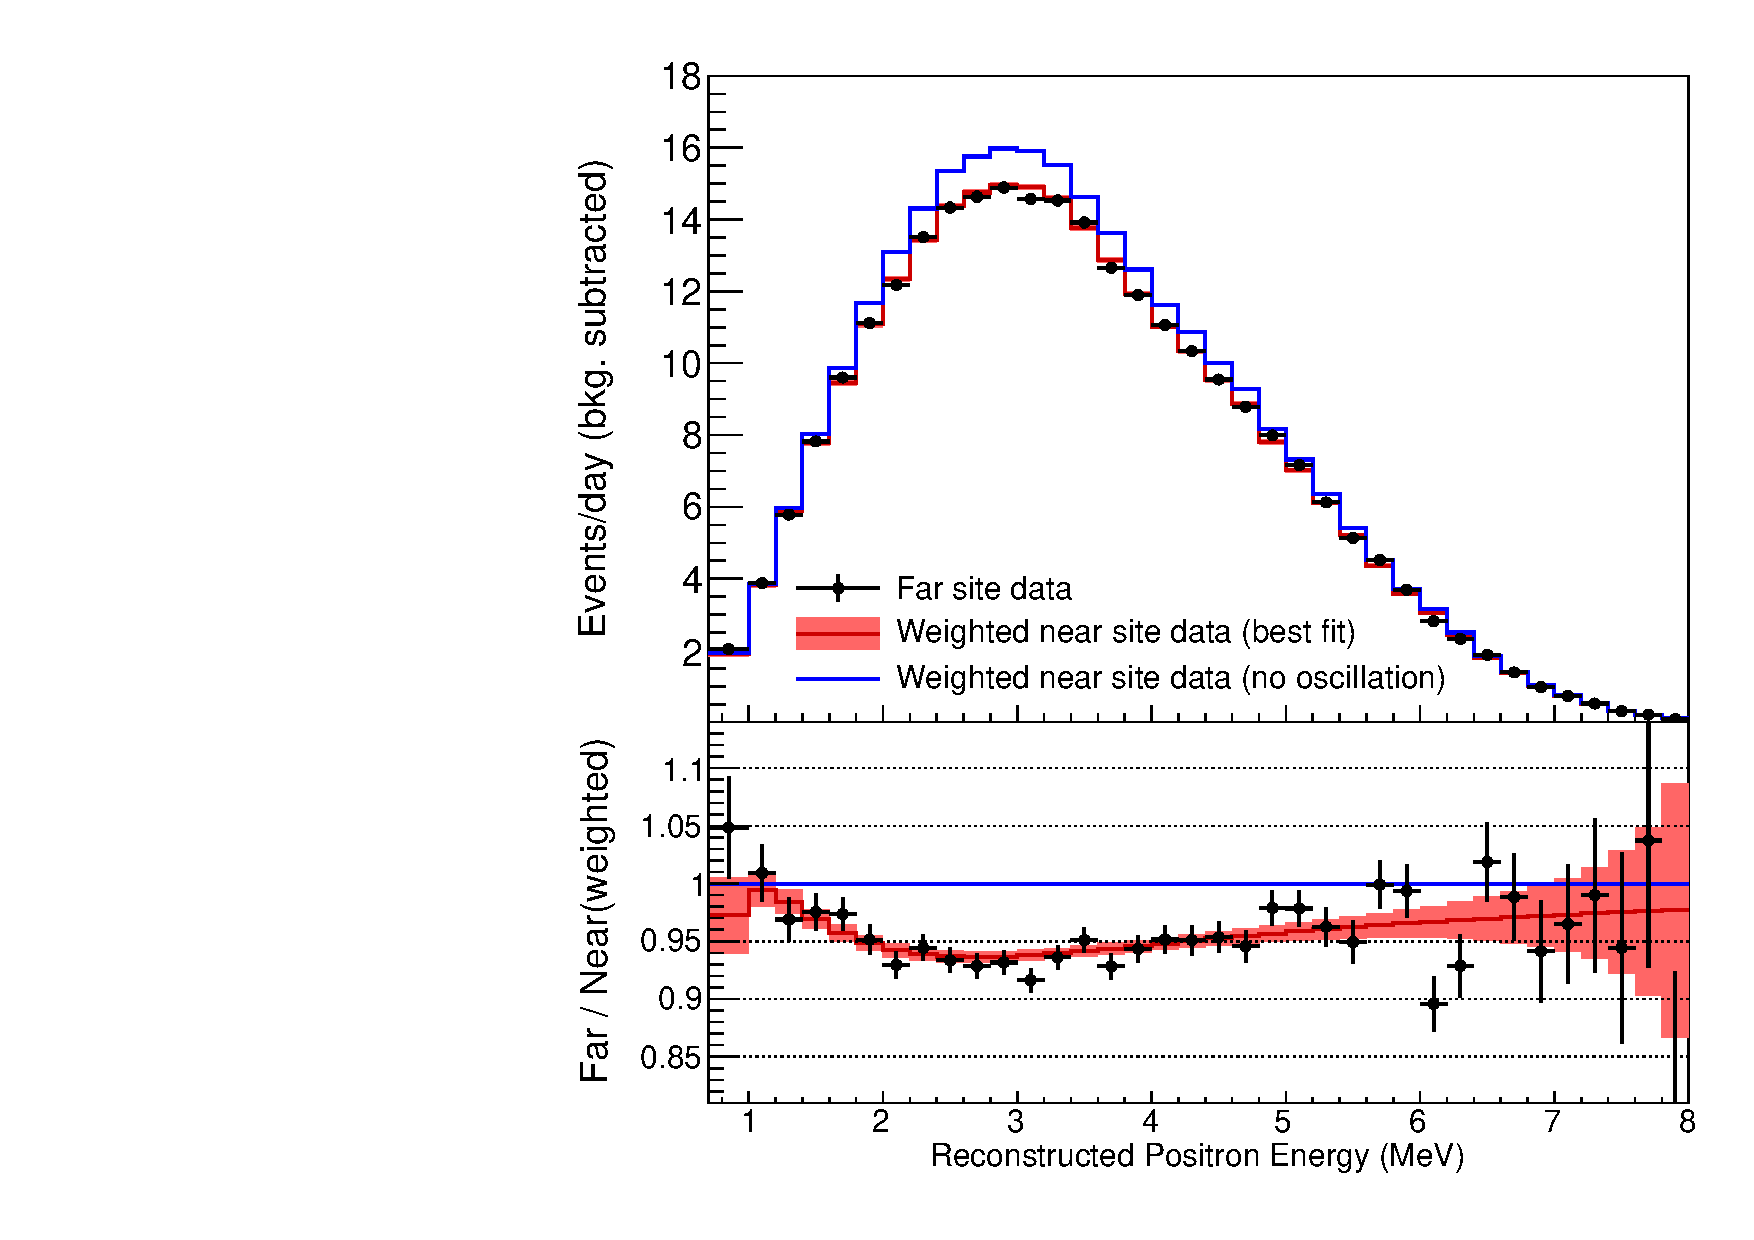
\includegraphics[width=0.9\linewidth]{figures/spectral_distortion_NL2015_v2.pdf}
   \end{minipage} \hfill
   \begin{minipage}{.46\linewidth}
      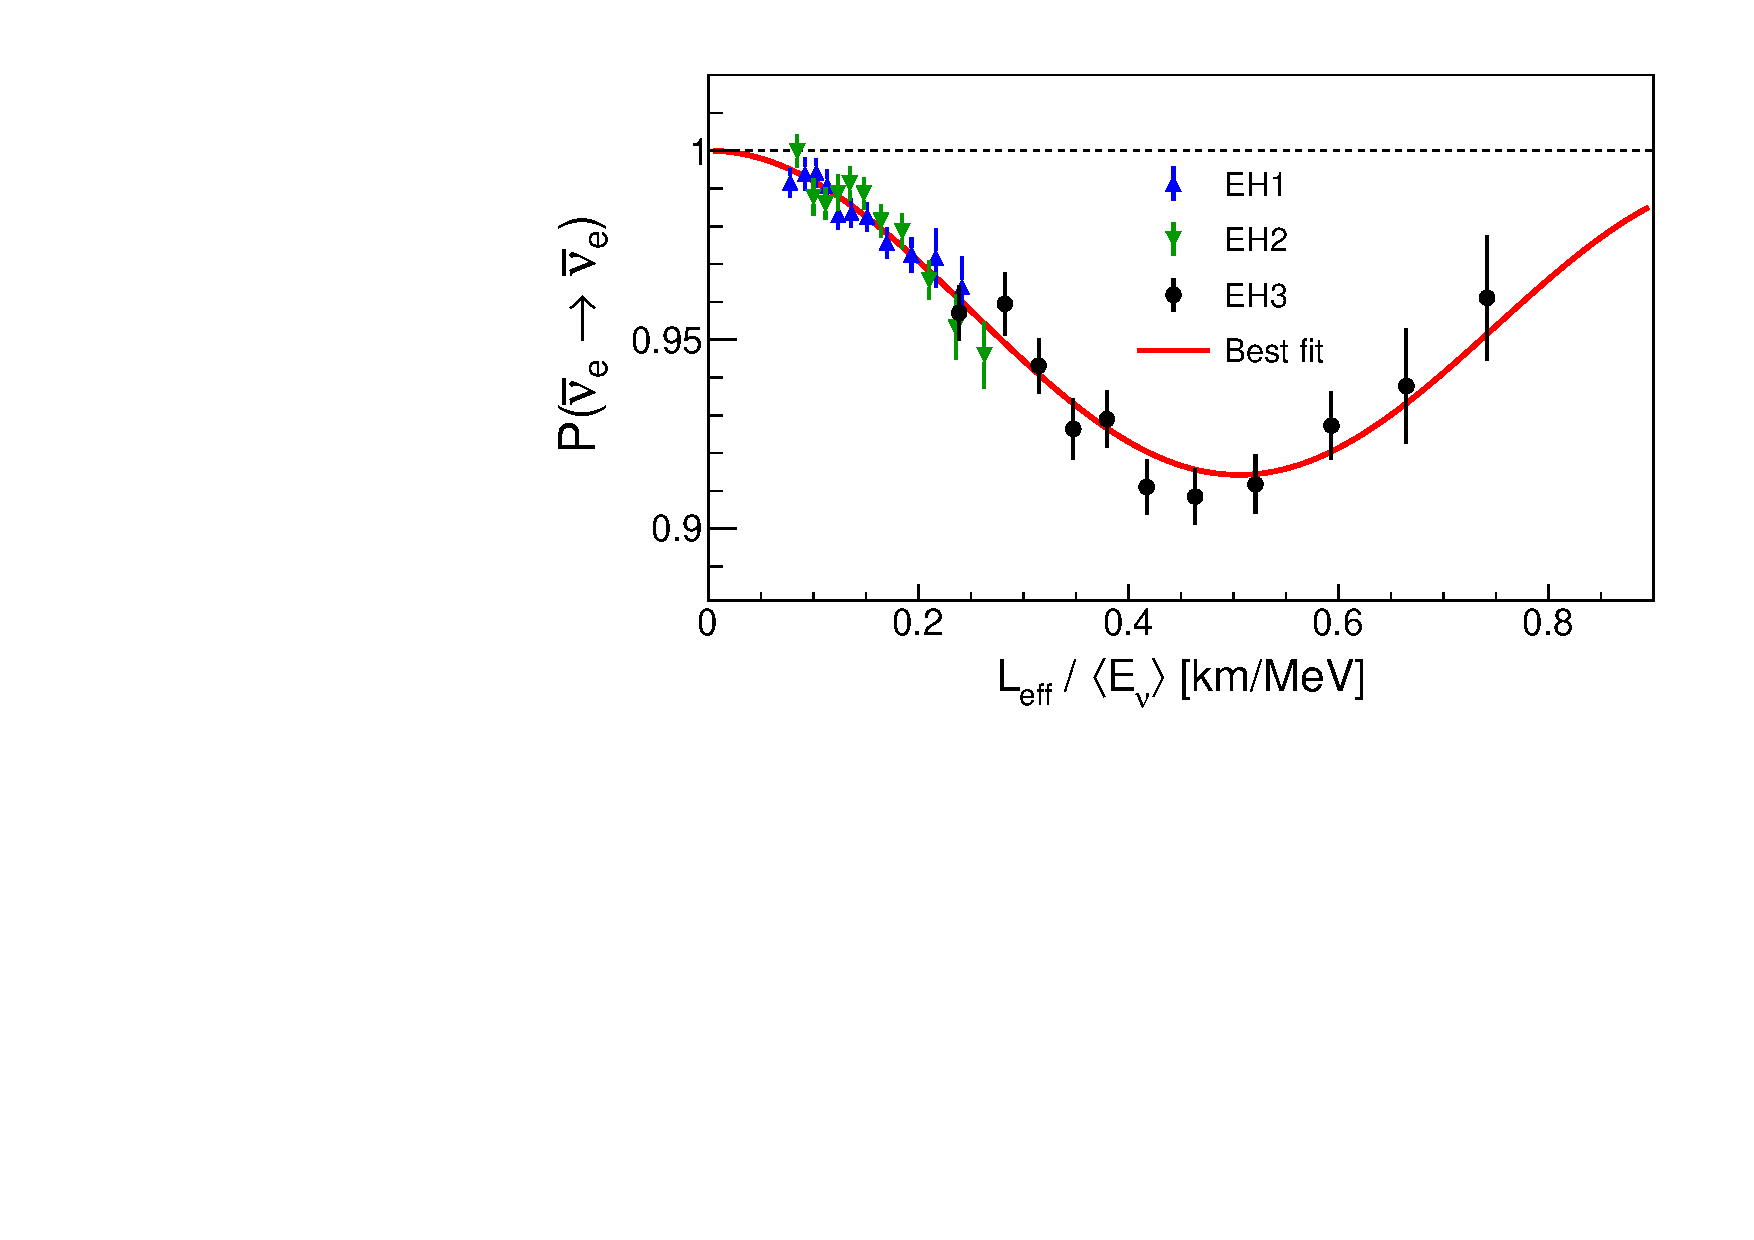
\includegraphics[width=0.9\linewidth]{figures/loe_NL2015.pdf}
   \end{minipage}
    \caption{Left plot: the reconstructed positron
energy spectrum observed by Daya Bay in the far site (black points), 
the expectation derived from the near sites without(blue line) or
with (red line) oscillation. The lower plot shows the ratio of the spectra to the no-oscillation case and the shaded area 
includes the systematic and statistical uncertainties~\cite{An:2015rpe}. 
Right plot: Daya Bay electron antineutrino survival probability versus effective
propagation distance L divided by the average antineutrino energy
E~\cite{An:2015rpe}.
}
 \label{fig:dayabay}
\end{figure}



%(a mettre dans la partie anomalies)
%Recently (ref Mueller, Huber) the total IBD rate of reactor neutrino experiments has been recomputed and found to predict xx \% more events than observed. This has initiated the so-called "reactor neutrino anomaly". 
%If this anomaly is interpreted as due to neutrino oscillations, it would imply the mixing of $\bar{\nu}_e$ with a new sterile neutrino state with a mass around 1 eV, as the deficit is already apparent at a distance of 10 m from the reactor core. 
%A new generation of experiment is currently being constructed or in data-taking to probe this anomaly. It includes reactor experiments very close to the reactor core (STEREO, SOLID, DANSS, NEUTRINO-4) or with an intense antineutrino source (SOX). These experiments aim to observe a deformation of the spectrum if the hypothesis of oscillation is correct. They will release results with a very short timescale, starting in 2017 (to be checked).  
%

